\begin{frame}
  \begin{center}
    \LARGE <<Интересные конкурсы>>
  \end{center}

  \begin{itemize}
  \item Идея задачи --- Григорий Резников
  \item Разработка задачи --- Максим Деб Натх
  \end{itemize}

\end{frame}

\begin{frame}{Постановка задачи}

  \begin{itemize}
  \item Дана скобочная последовательность
  \item За $t$ времени можно перемешать любой её подотрезок длины $t$
  \item Нужно за минимальное время сделать последовательность правильной скобочной
  \end{itemize}
  
\end{frame}

\begin{frame}{Ответ отрицательный}
  \begin{itemize}
  \item Поймём, когда мы не можем сделать последовательность ПСП
  \item Тогда и только тогда, когда число \texttt{<<(>>} и число \texttt{<<(>>} в строке отличается
  \item Иначе всегда можно взять всю строку и переставить в ней за $n$ символы так, чтобы строка стала ПСП, например, \texttt{<<(((($\dots$))))>>}
  \end{itemize}
\end{frame}

\begin{frame}{Основная идея}
  \begin{itemize}
  \item Заметим, что в оптимальном решении отрезки, на которых производятся перемешивания не пересекаются (иначе можно было перемешать сразу нормально)
  \item Значит для перемешивания нужно выбрать набор непересекающихся отрезков.
    \bigskip
  \item Скобочный баланс -- разность между количеством \texttt{<<(>>} и количеством \texttt{<<)>>}
  \item За $bal_i$ ($0 \le i \le n$) обозначим скобочный баланс на первых $i$ символах.
  \end{itemize}
\end{frame}

\begin{frame}{Решение за $\mathcal{O}(n^2)$ (50 баллов)}
  \begin{itemize}
  \item Используем динамику $dp_i=$ сколько времени нужно, чтобы сделать префикс из $i$ символов префиксом ПСП
  \item $dp_0 = 0, dp_i = -\infty$, если $bal_i < 0$, иначе

    \[ dp_i = \min \left\{
    \begin{array}{ll}
      dp_{i-1} & \textrm{если } bal_i \geq 0 \\
      j + dp_{i-j} & \textrm{по всем } j \leq i \textrm{ таким, что } \\
      & bal_i \leq bal_{i-j}
    \end{array} \right. \]
  \end{itemize}
\end{frame}

\begin{frame}{Полное решение за $\mathcal{O}(n)$}
  \begin{itemize}
    %% \item Рассмотрим такой индекс $i$, что что $bal_{i-1} \leq 0$, $bal_{i} < 0$, либо $bal_{i-1} < 0$, $bal_i \leq 0$. Тогда, если символ $s_i$ не будет участвовать ни в одном перемешивании, то итоговая строка будет иметь $i$-й или $i-1$-й префиксный баланс отрицательным
    %%  \item Изобразим данную с.п. как ломанную. Описанные выше индексы~--- это все отрезки ниже линии $x=0$

  \item Изобразим скобочную последовательность графически:

    \begin{figure}[htb]
      \centering
      \resizebox{0.6\textwidth}{!}{
        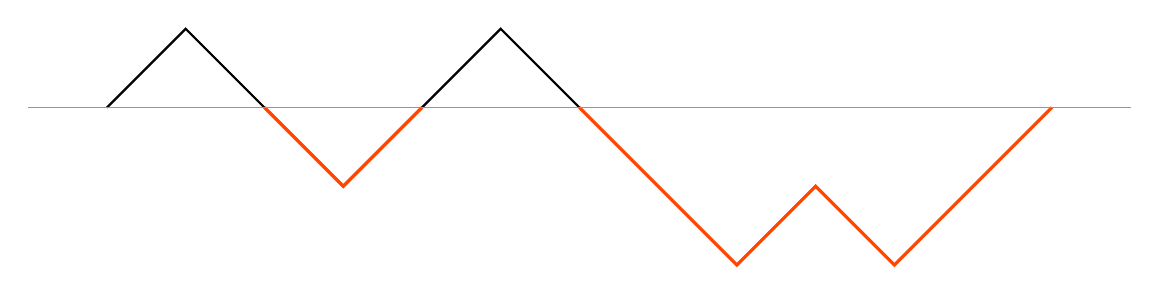
\begin{tikzpicture}
          \draw [OrangeRed, very thick] (0,0) -- ++(1,-1) -- ++(1, 1);
          \draw [thick] (2,0) -- ++(1,1) -- ++(1,-1);
          \draw [OrangeRed, very thick] (4,0) -- ++(1,-1) -- ++(1, -1) -- ++(1, 1) -- ++(1, -1) -- ++(1, 1) -- ++(1, 1);
          \draw [thick] (-2,0) -- ++(1,1) -- ++(1,-1);
          \draw [green] (-3, 0) -- (+11, 0);
      \end{tikzpicture}}%
      \caption{ПСП до перемешиваний}
    \end{figure}

    Видно, что если взять все последовательности красных скобок и развернуть их, получим ПСП:
    \begin{figure}[htb]
      \centering
      \resizebox{0.6\textwidth}{!}{
        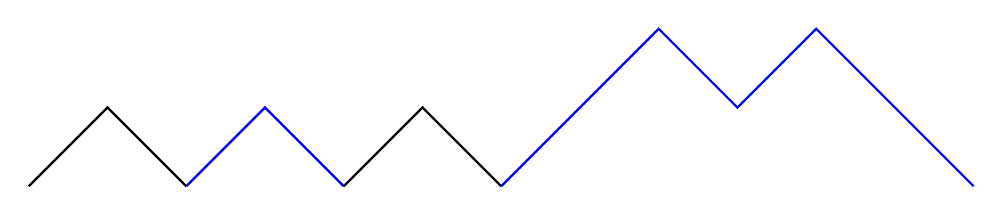
\begin{tikzpicture}
          \draw [blue, thick] (0,0) -- ++(1,1) -- ++(1, -1);
          \draw [thick] (2,0) -- ++(1,1) -- ++(1,-1);
          \draw [blue, thick] (4,0) -- ++(1,1) -- ++(1, 1) -- ++(1, -1) -- ++(1, 1) -- ++(1, -1) -- ++(1, -1);
          \draw [thick] (-2,0) -- ++(1,1) -- ++(1,-1);
      \end{tikzpicture}}%
      \caption{ПСП после перемешиваний}
    \end{figure}
  \end{itemize}
\end{frame} 

\begin{frame}{Полное решение за $\mathcal{O}(n)$}
  \begin{itemize}
  \item Значит, достаточно найти число скобок <<ниже нулевого баланса>>, их количество и будет ответом.
  \end{itemize}
\end{frame} 
